\part{De la programmation visuelle à la programmation textuelle}
\chap{Apprendre le langage AESL à partir des programmes VPL}\label{ch.next}

Félicitations!
Vous êtes expert(e) de la programmation visuelle (VPL).
Vous pouvez maintenant vous lancer dans la programmation textuelle
avec l'\textit{environnement de programmation Studio} et son langage de
programmation, l'\textit{Aseba Event Scripting Language (AESL)}.


\begin{figure}[hbt]
\begin{center}
\gr{studio}{.8}
\caption{L'environnement d'Aseba Studio}\label{fig.studio}
\end{center}
\end{figure}

VPL traduit les programmes graphiques (les paires événement-actions) en programmes textuels AESL
qui apparaîssent d'ailleurs sur le côté droit de la fenêtre VPL (numéro~6 dans la \cref{fig.vplgui}
de la page~\pageref{fig.vplgui}).
Ce tutoriel utilise des programmes VPL des chapitres précédents et décrit leur programme AESL correspondant.
Vous utiliserez vos connaissances de ces programmes VPL pour apprendre les principes fondamentaux 
de la programmation AESL.

La programmation utilisant Aseba Studio est aussi basée sur les concepts d'événements et d'actions.
Comme les programmes VPL sont traduits en programmes AESL,
tout ce que vous avez appris dans ce tutoriel est aussi disponible dans Studio,
mais vous avez maintenant la flexibilité d'un langage de programmation complet
avec des variables, des expressions et des structures de contrôle.

Lorsque vous travaillez dans Aseba Studio, vous pouvez ouvrir VPL en cliquant sur le bouton
\bu{Lancer VPL} dans l'onglet \emph{Outils} en bas à gauche de la fenêtre.
Vous pouvez importer des programmes VPL vers Aseba Studio simplement en ouvrant le fichier du programme.

Les sections avec une $^*$ présentent des concepts de la programmation AESL qui dépassent les 
possibilités de VPL.
Elles peuvent être sautées si vous lisez ce tutoriel pour la première fois.

\newpage

\textbf{\large Documentation}

Pour en savoir plus sur Aseba Studio et AESL, rendez-vous sur la page \emph{Programmer avec du texte}
disponible sur \href{https://www.thymio.org/fr:asebausermanual}{https://www.thymio.org/fr:asebausermanual}.
Vous y trouverez la documentation concernant:

\begin{itemize}
\item L'environnement de programmation Studio
\item Le langage de programmation AESL
\item L'interface pour le robot Thymio.
(il existe une feuille de référence pour l'interface).
\item La bibliothèque contenant toutes les fonctions natives présentes dans AESL.
\end{itemize}

Il y a aussi une archive qui propose différents projets intéressants à réaliser avec AESL
avec le code source de la solution proposée.

\sect{L'interface du Thymio}

Voici le programme \p{whistles.aesl} du \cref{ch.bells} avec une partie du programme AESL correspondant:

\begin{center}
\begin{tabular}{ll}
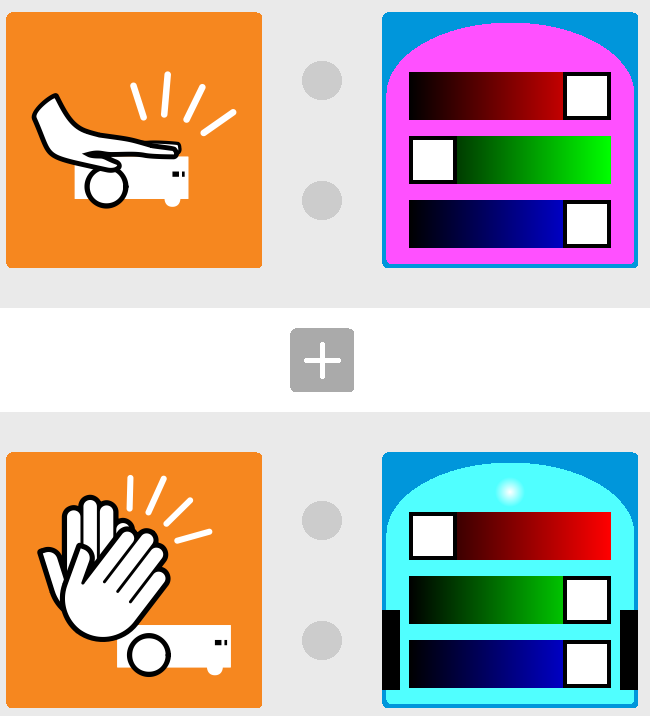
\includegraphics[width=.4\textwidth]{whistles} &
\begin{minipage}[b]{.5\textwidth}
\begin{footnotesize}
\begin{verbatim}
  onevent tap
    call leds.top(32,0,32)
  
  onevent mic
    call leds.bottom.left(0,32,32)
    call leds.bottom.right(0,32,32)
\end{verbatim}
\end{footnotesize}
\vspace*{8ex}
\end{minipage}
\end{tabular}
\end{center}

\textbf{\large Traitement des événements}

Lorsqu'un événement tape est déclenché, la lumière du haut est allumée en une couleur appelée
\emph{magenta},
et lorsqu'un événement frapper des mains est déclenché, la lumière du bas est allumée en une couleur 
appelée \emph{cyan}.
Dans AESL, ce qui correspond aux paires événement-actions de VPL est un système de traitement des événements
qui est introduit par le mot-clé \p{onevent} (en anglais, \emph{on event} signifie <<\,lors de l'événement\,>>)
Vous trouverez une liste des événements dans la table au bas de la documentation pour l'interface
de programmation de Thymio.

Les lignes qui suivent \p{onevent} forment le corps principal du traitement de l'événement \p{tap}, respectivement \p{mic}.
Ils correspondent aux blocs action à droite des blocs événement dans VPL.

Lorsqu'un événement tape est déclenché, la \emph{fonction d'interface} \p{leds.top} est \emph{appelée}.
La fonction prend trois \emph{paramètres} qui spécifient l'intensité de rouge, de vert et de bleu de la LED.
Les valeurs de celles-ci varient entre 0 (éteinte) et 32 (complètement allumée).
Combiner du rouge et du bleu permet d'obtenir du magenta.

L'événement VPL frapper dans les mains correspond à l'événement \p{mic} (une forme abrégée pour 
microphone).
Lorsque l'événement est déclenché, les LEDs du bas sont allumées.
Dans VPL, un bloc action allume les deux LEDs de la même couleur
alors que dans AESL, les LEDs droite et gauche peuvent être allumées indépendamment l'une de l'autre.
Dans notre cas, nous allumons les deux LEDs avec les composantes vertes et bleues à pleine intensité,
ce qui donne du cyan.

\textbf{\large Affecter une valeur à une variable}

Regardez à nouveau le programme AESL dans la fenêtre VPL.
Les deux premières lignes sont:

\begin{footnotesize}
\begin{verbatim}
  # setup threshold for detecting claps
  mic.threshold = 250
\end{verbatim}
\end{footnotesize}

Une ligne qui commence avec un \verb+#+ est appelée un \emph{commentaire}.
Les commentaires n'ont aucune influence sur le programme;
on les utilise pour donner des informations au lecteur du programme.
Dans ce cas, le commentaire explique que l'événement frapper les mains 
est déclenché lorsque l'intensité du son est plus grande qu'un certain
\emph{seuil}.
La deuxième ligne du programme spécifie que l'événement est déclenché lorsque l'intensité du son
(qui est entre $0$ et $255$) est plus grand que $250$.

Dans VPL, ce seuil est intégré à l'événement et il ne peut pas être changé,
mais dans un programme textuel, vous pouvez le changer en \emph{affectant} une valeur à une variable:

\begin{footnotesize}
\begin{verbatim}
  mic.threshold = 180
\end{verbatim}
\end{footnotesize}

Ceci signifie que la \emph{valeur} à droite du \verb+=+ est copiée vers la \emph{variable}
à gauche.
La variable \p{mic.threshold} est prédéfinie pour le robot Thymio.

\textbf{\large Initialisation du Thymio}

Au début de chaque programme,
VPL insère automatiquement une suite d'instructions 
pour éteindre toutes les LEDs et le son.

\begin{footnotesize}
\begin{verbatim}
    # reset outputs
    call sound.system(-1)
    call leds.top(0,0,0)
    call leds.bottom.left(0,0,0)
    call leds.bottom.right(0,0,0)
    call leds.circle(0,0,0,0,0,0,0,0)
\end{verbatim}
\end{footnotesize}

Cette \emph{initialisation} n'est pas visible dans le programme VPL.
Dans un programme textuel, nous recommandons d'inclure ces instructions,
bien qu'elles ne soient pas nécessaires.

\newpage

\sect{Plusieurs alternatives}

Le programme \p{colors-multiple.aesl} du \cref{ch.colors} change
la couleur des LEDs du haut et du bas lorsque les boutons sont touchés:

\begin{center}
\begin{tabular}{ll}
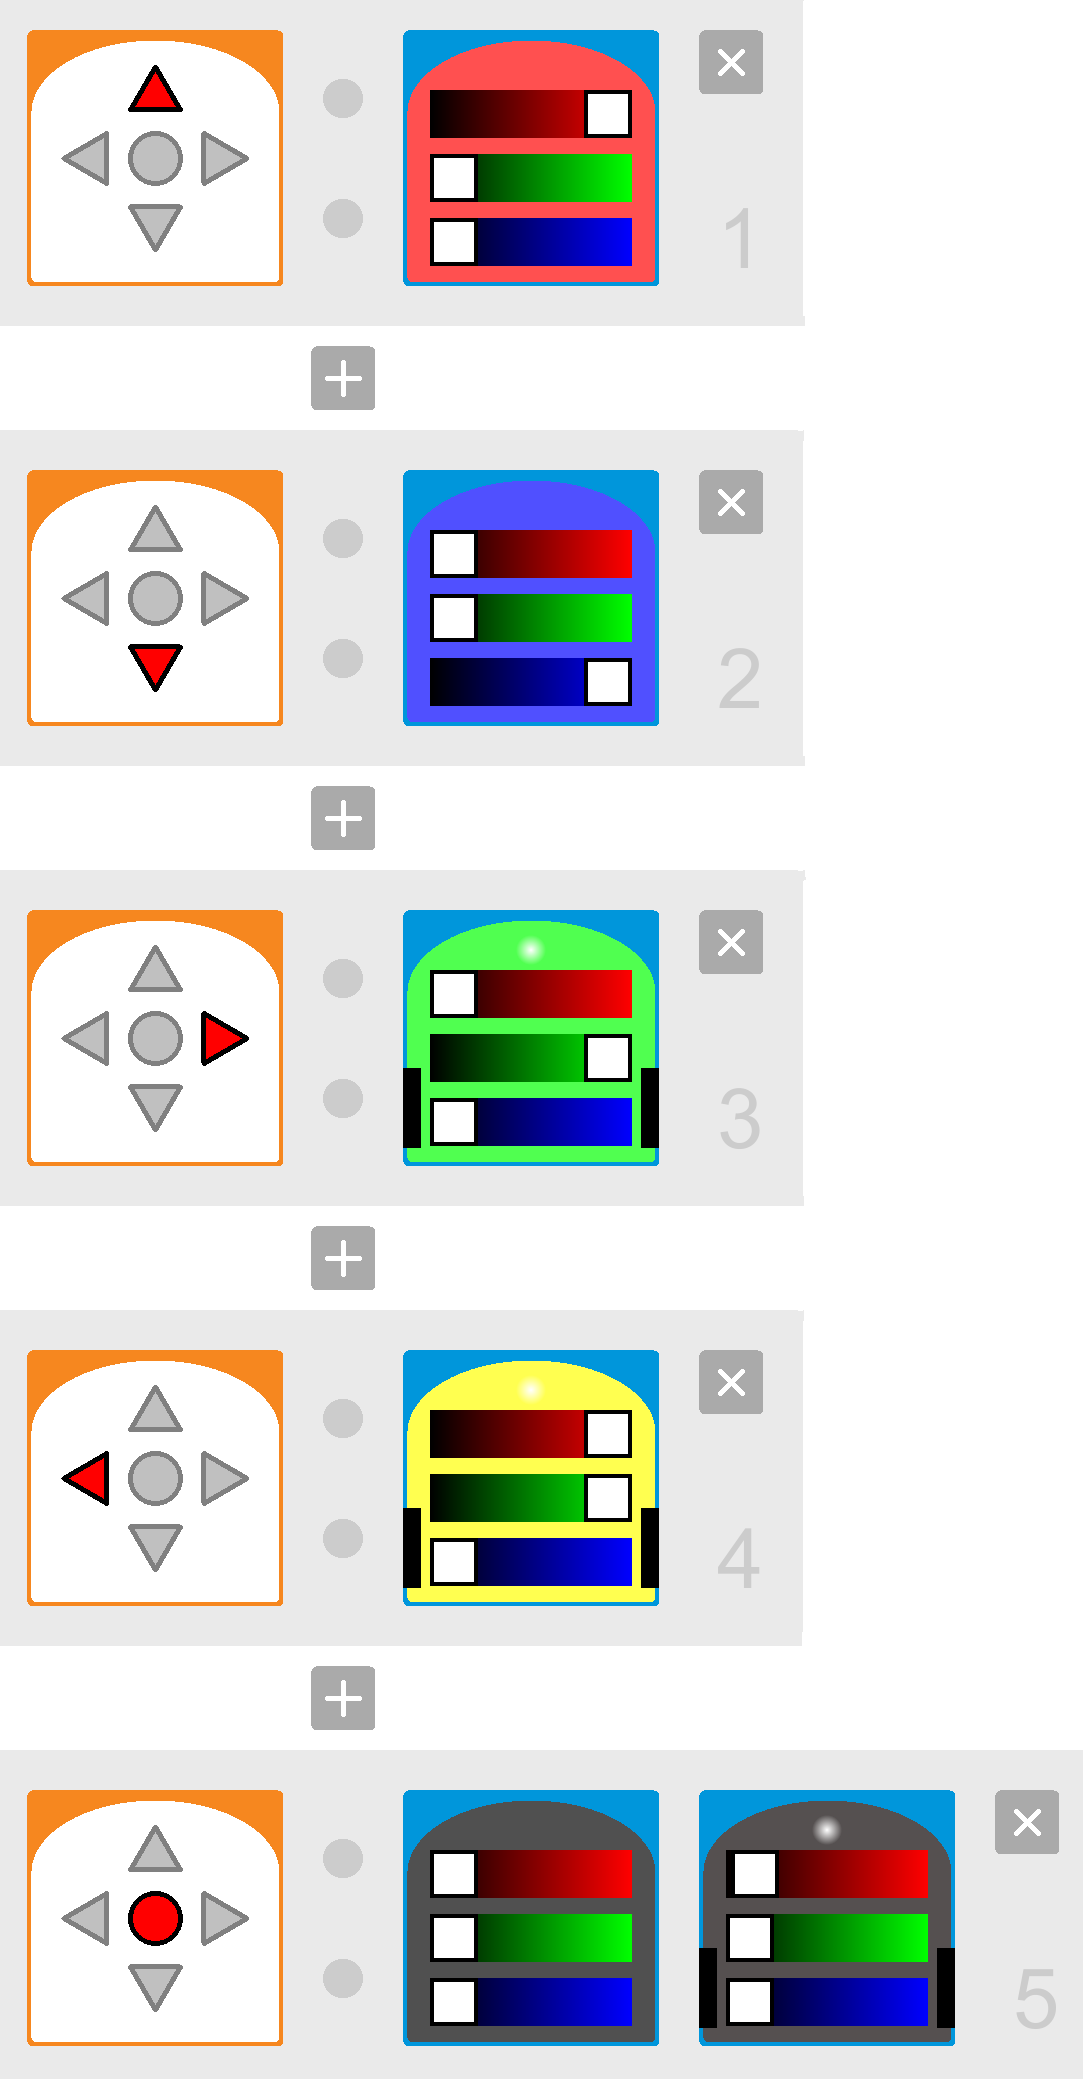
\includegraphics[width=.4\textwidth]{colors-multiple-full} &
\begin{minipage}[b]{.5\textwidth}
\begin{footnotesize}
\begin{verbatim}
  onevent buttons
    when button.forward == 1 do
      call leds.top(32,0,0)
    end
    when button.backward == 1 do
      call leds.top(0,0,32)
    end
    when button.right == 1 do
      call leds.bottom.left(0,32,0)
      call leds.bottom.right(0,32,0)
    end
    when button.left == 1 do
      call leds.bottom.left(32,32,0)
      call leds.bottom.right(32,32,0)
    end
    when button.center == 1 do
      call leds.top(0,0,0)
      call leds.bottom.left(7,0,0)
      call leds.bottom.right(7,0,0)
    end
\end{verbatim}
\end{footnotesize}
\vspace*{5ex}
\end{minipage}
\end{tabular}
\end{center}

Dans le programme AESL, \emph{un seul} événement est déclenché chaque fois qu'un des cinq boutons
est touché.
L'action du traitement d'événement introduit par \p{onevent buttons}
dépend du bouton touché. Nous allons donc nous référer à la valeur des \emph{variables bouton}
pour sélectionner l'action à exécuter.
Les instructions:

\begin{footnotesize}
\begin{verbatim}
  when button.forward == 1 do
    call leds.top(32,0,0)
  end
\end{verbatim}
\end{footnotesize}

signifient: \emph{quand} (<<\,when\,>> signifie <<\,quand\,>> en anglais) la valeur de la variable \p{button.forward} (\emph{button.forward} signifie
<<\,bouton.avant>> en anglais) est un,
\emph{alors} exécute les actions écrites entre les mots-clés \p{do} (qui signifie <<\,exécute\,>> en anglais)
et \p{end} (qui signifie <<\,fin\,>> en anglais).
Il y a cinq variables \p{bouton}, une pour chacun des boutons.
La valeur d'une variable bouton vaut 1 si le bouton est touché et 0 si le bouton est relâché.
Dans ce programme, il y a cinq structures introduites par \p{when}, une pour chaque bouton.
Une ou deux actions sont exécutées si l'expression dans une structure \p{when} \emph{devient} vraie.

\informationbox{La programmation textuelle et l'anglais}{
La grande majorité -- si ce n'est la totalité -- des langages de programmation utilisent 
des mots-clés en anglais, la langue de référence pour les codeurs du monde entier.
Ainsi, nous avons déjà vu les mots-clés \p{onevent}, \p{when}, \p{do} et \p{end}
qui nous viennent tous de l'anglais. Nous en verrons encore quelques autres.
Si vous ne comprenez pas l'anglais, il vous faudra mémoriser ces quelques mots,
mais, rassurez-vous, ils ne sont pas nombreux.}

\textbf{\large Un ou plusieurs événements$^*$}

L'interface Thymio inclut aussi des événements distincts pour chaque bouton,
en plus de l'événement \p{buttons} qui est déclenché chaque fois qu'un bouton est pressé ou relâché.
Nous pourrions aussi implémenter ce programme avec de multiples événements et sans structures
\p{when} ni variables bouton:

\begin{footnotesize}
\begin{verbatim}
  onevent button.forward
    call leds.top(32,0,0)
  
  onevent button.backward
    call leds.top(0,0,32)
  
  onevent button.right
    call leds.bottom.left(0,32,0)
    call leds.bottom.right(0,32,0)
  
  onevent button.left
    call leds.bottom.left(32,32,0)
    call leds.bottom.right(32,32,0)
  
  onevent button.center
    call leds.top(0,0,0)
    call leds.bottom.left(1,0,0)
    call leds.bottom.right(1,0,0)
\end{verbatim}
\end{footnotesize}

Utiliser des événements distincts a l'avantage d'être plus facile à lire et à comprendre.
Néanmoins, dans les cas de figure suivants, l'utilisation de l'événement \p{buttons} est nécessaire:
(a) pour pouvoir faire la différence entre un bouton touché et un bouton relâché
et
(b) pour détecter que deux boutons sont touché en même temps:

\begin{footnotesize}
\begin{verbatim}
  onevent buttons
    # Allumez les LEDs du haut lorsque le bouton avant est relâché
    when button.forward == 0 do
      call leds.top(32,0,0)
    end

    # Allumez les LEDs du bas lorsque à la fois
    # les boutons gauche et droite sont pressés
    when button.left == 1 and button.right == 1 do
      call leds.bottom.left(0,32,0)
      call leds.bottom.right(0,32,0)
    end
\end{verbatim}
\end{footnotesize}

Une autre différence est que les événements spécifiques à un bouton
ont lieu lorsqu'un bouton est touché ou relâché,
tandis que l'événement commun à tous les boutons est déclenché à une fréquence de 20 Hz,
à chaque fois que le tableau des variables bouton est mis à jour (voir page~\pageref{pg.hz}
pour une explication de ces concepts).

\textbf{\large Structures \p{if}}

AESL supporte deux structures différentes:
\begin{footnotesize}
\begin{verbatim}
  when v == 1 do ... instructions ... end

  if v == 1 then ... instructions ... end
\end{verbatim}
\end{footnotesize}
qui ont des significations différentes (<<\,if ... then\,>> signifie <<\,si ... alors\,>>, tandis que nous avons déjà vu que <<\,when ... do\,>> signifie <<\,quand ... exécute\,>>):
\begin{quote}
\emph{quand} la valeur de \p{v} \emph{devient} 1, exécute les instructions\\
\emph{si} la valeur de \p{v} \emph{est} 1, exécute les instructions
\end{quote}

Les structures \p{when} s'utilisent en général pour des variables qui représentent des événements
parce que souvent on souhaite réagir quand un événement est déclenché et non pas simplement quand une variable a une certaine valeur.
On pourrait réagir à un événement \p{buttons} en utilisant une structure \p{if}:

\begin{footnotesize}
\begin{verbatim}
  onevent buttons
    if button.forward == 1 then
      ... instructions ...
    end
\end{verbatim}
\end{footnotesize}
Néanmoins, si nous gardons le bouton avant appuyé pendant assez longtemps,
ces instructions seraient exécutées plusieurs fois.
Si les instructions changent la couleur des LEDs, on ne voit aucune différence, mais
dans certains cas, il y a une différence et la structure \p{when} est alors nécessaire.

Une structure \p{if} est plus appropriée lorsque ce qui nous intéresse est la valeur d'une variable
et non le changement de cette valeur.
Les instructions suivantes attribuent la valeur mesurée maximale entre les deux capteurs arrières à la variable \p{max}:

\begin{footnotesize}
\begin{verbatim}
  if prox.horizontal[5] > prox.horizontal[6] then
    max = prox.horizontal[5]
  else
    max = prox.horizontal[6]
  end
\end{verbatim}
\end{footnotesize}

Nous verrons des exemples supplémentaires de structures \p{if} dans la section suivante et
dans la Figure~\ref{fig.respond}.


\newpage



\sect{Les tableaux}

Le programme \p{likes.aesl} dans le \cref{ch.pet} du tutoriel VPL
permet au robot de suivre votre main alors que vous la bougez d'un côté à l'autre de l'avant du robot,
en face des capteurs de proximité avants.
Lorsqu'aucun objet n'est détecté, le robot s'arrête;
lorsqu'un objet est détecté devant le capteur central, le robot avance;
lorsqu'un objet est détecté devant le capteur tout à gauche ou tout à droite,
le robot tourne dans cette direction.

\begin{figure}[hbt]
\begin{center}
\begin{tabular}{lr}
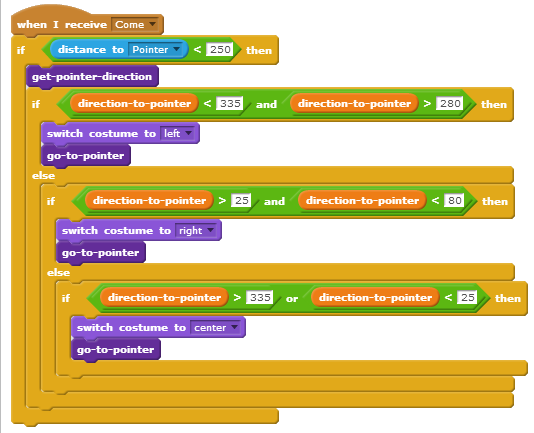
\includegraphics[width=.35\textwidth]{likes} &
\begin{minipage}[b]{.4\textwidth}
\begin{footnotesize}
\begin{verbatim}
  onevent prox
    when prox.horizontal[2] < 1000 do
      motor.left.target = 0
      motor.right.target = 0
    end
    when prox.horizontal[2] > 2000 do
      motor.left.target = 300
      motor.right.target = 300
    end
    when prox.horizontal[0] > 2000 do
      motor.left.target = -300
      motor.right.target = 300
    end
    when prox.horizontal[4] > 2000 do
      motor.left.target = 300
      motor.right.target = -300
    end
\end{verbatim}
\end{footnotesize}
\end{minipage}
\end{tabular}
\caption{The \p{likes} program in VPL and AESL}\label{fig.arrays}
\end{center}
\end{figure}

La structure du programme AESL (\cref{fig.arrays}) contient un traitement d'événements
avec plusieurs structures \p{when}.
Les valeurs de la position des \textit{sliders} des blocs moteurs sont affectés aux
variables moteur correspondantes \p{motor.left.target} et \p{motor.right.target}
(qui signifient respectivement <<\,moteur.gauche.cible>> et <<\,moteur.droit.cible>>).
Dans VPL, les \textit{sliders} permettent de modifier les valeurs des variables moteur
par incréments de $50$, mais AESL vous permet d'affecter toutes les valeurs dans l'intervalle 
$-500$ à $500$.

L'événement est appelé \p{prox} (une forme abrégée pour <<\,proximité\,>>).
Contrairement aux événements bouton qui sont déclenchés lorsque quelque chose <<\,se produit\,>>,
cet événement est déclenché \emph{10 fois par seconde}.
Avant que l'événement ne se produise, des valeurs qui dépendent de ce qui est détecté par les capteurs
sont affectées aux variables \p{prox.horizontal}.
Voir la documentation\label{pg.hz} de l'interface de programmation Thymio pour plus de détails.
\footnote{L'unité de mesure pour la \emph{fréquence}, le nombre de fois que quelque chose 
se produit par seconde est le \emph{hertz}, que l'on abrège \emph{Hz}.
La documentation de l'interface précise que l'événemnet {\footnotesize\p{prox}} se produit
à une fréquence de \emph{10 Hz}.}

\textbf{\large Des tableaux comme variables multiples}

Le robot Thymio a sept capteurs de proximité horizontaux, 5 à l'avant et 2 à l'arrière.
Pour lire les valeurs mesurées par les capteurs, on pourrait définir 7 variables différentes:

\begin{footnotesize}
\begin{verbatim}
  prox.horizontal.front.0
  prox.horizontal.front.1
  prox.horizontal.front.2
  prox.horizontal.front.3
  prox.horizontal.front.4
  prox.horizontal.back.0
  prox.horizontal.back.1
\end{verbatim}
\end{footnotesize}

Mais au lieu de faire ainsi, AESL permet de définir des \emph{tableaux}, des suites
de variables qui ont toutes le même nom.
Les différentes variables sont identifiées avec un nombre pour pouvoir les différencier.
Un tableau pour les capteurs de proximité horizontaux est prédéfini est porte le nom \p{prox.horizontal}:

\begin{center}
\begin{picture}(240,40)
\put(0,0){\makebox(100,20)[l]{\p{prox.horizontal}}}
\put(100,0){\framebox(140,20){}}
\multiput(120,0)(20,0){6}{\line(0,1){20}}
\put(100,20){\makebox(20,20){\p{0}}}
\put(120,20){\makebox(20,20){\p{1}}}
\put(140,20){\makebox(20,20){\p{2}}}
\put(160,20){\makebox(20,20){\p{3}}}
\put(180,20){\makebox(20,20){\p{4}}}
\put(200,20){\makebox(20,20){\p{5}}}
\put(220,20){\makebox(20,20){\p{6}}}
\end{picture}
\end{center}

Les 5 premières entrées du tableau correspondent aux capteurs avant, de gauche à droite.
Les 2 dernières correspondent aux capteurs arrières, de gauche à droite.
Si vous ne vous rappelez plus de la numérotation, vous pouvez toujours la retrouver 
dans la documentatoin de l'interface de programmation Thymio.
Encore mieux, vous la trouvez aussi sur le diagramme de la petite carte de référence.

Pour accéder à une entrée particulière du tableau, écrivez son numéro entre crochets à la fin 
du nom du tableau. On appelle ce nombre son \emph{indice} dans le tableau.
L'instruction suivante indique que les variables moteur seront mises à 300 lorsque la valeur du \emph{capteur
avant central} (indice 2) devient supérieure à 2000:

\begin{footnotesize}
\begin{verbatim}
  when prox.horizontal[2] > 2000 do
    motor.left.target = 300
    motor.right.target = 300
  end
\end{verbatim}
\end{footnotesize}

Nous verrons plus tard que l'on peut affecter des valeurs à des variables tableau:
\begin{footnotesize}
\begin{verbatim}
  timer.period[0] = 1979
\end{verbatim}
\end{footnotesize}

\textbf{\large Les boucles \p{for} et les variables d'indices$^*$}

Une généralisation naturelle des tableaux consiste en l'utilisation d'une variable au lieu du
constante comme indice.\footnote{Ceci n'est pas utilisé dans les programmes VPL traduits en AESL,
à part dans un cas complexe de création de sons; c'est pourquoi l'exemple ici est repris des projets
AESL.}
Le programme \p{cats.aesl} contient l'instruction suivante:

\begin{footnotesize}
\begin{verbatim}
  var i

  for i in 0:4 do
    if prox.horizontal[i] > DETECTION then
      state = 2
    end
  end
\end{verbatim}
\end{footnotesize}

Précédemment, nous avons utilisé uniquement les variables comprises dans l'interface Thymio;
ici, la première ligne \emph{déclare} une nouvelle variable appelée \p{i}.
L'instruction suivante est une boucle \p{for} (de l'anglais <<\,pour\,>>. Le mot-clé \p{in} signifie <<\,dans\,>>) dont la signification est: 

\begin{itemize}
\item Affecter les valeurs 0, 1, 2, 3, 4 à tour de rôle à la variable \p{i};
\item Pour chacune des affectations, exécuter les actions entre \p{do} (<<\,faire\,>> en anglais)
    et \p{end} (<<\,fin\,>> en anglais).
\end{itemize}

Ici, nous n'avons qu'une seule structure \p{if} entre \p{do} et \p{end}.
Elle vérifie la valeur des capteurs de proximité centraux et affecte la valeur 2 à la variable
\p{state} si la valeur obtenue d'un des capteurs est plus grande que la constante \p{DETECTION}.
\footnote{Se référer à la documentation de l'environnement Aseba Studio pour les instructions
sur comment définir des constantes.}

La variable \p{i} prend à tour de rôle les valeurs 0, 1, 2, 3, 4.
Ainsi, chaque fois que la structure \p{if} est exécutée, \p{prox.horizontal[i]} retourne
la valeur mesurée par un capteur différent. Les valeurs de tous les capteurs de gauche à droite
sont ainsi lues.
Le résultat de la boucle \p{for} est donc d'affecter la valeur 2 à la variable \p{state}
\emph{si} \emph{un parmi} les capteurs avants détecte un objet.

\textbf{\large Déclarer un tableau}

Un tableau de variables se déclare en donnant sa taille entre crochet après le nom du tableau.
La taille peut aussi être donnée implicitement en donnant une valeur initiale au tableau:
\footnote{Un commentaire ne commence pas forcément au début d'une ligne.
Tout caractère entre le caractère \# et la fin de la ligne est considéré comme un commentaire et est ignoré par l'ordinateur.}

\begin{footnotesize}
\begin{verbatim}
var state[4] # Un tableau avec quatre éléments
var state[] = [0,0,0,0] # Un tableau avec quatre éléments
\end{verbatim}
\end{footnotesize}

Lors de la traduction du programme VPL, la taille et la valeur initiale est donnée.
Le code suivant est correct à condition que le nombre de valeur est égal à la taille indiquée:

\begin{footnotesize}
\begin{verbatim}
var state[4] = [0,0,0,0]
\end{verbatim}
\end{footnotesize}

\newpage

\sect{Les minuteurs}

Le \cref{ch.time} a présenté les \emph{minuteurs}.
Le programme \p{shy.aesl} demande au robot de tourner à gauche quand le capteur avant central
détecte votre main; deux secondes plus tard, il tourne à droite:

\begin{center}
\begin{tabular}{ll}
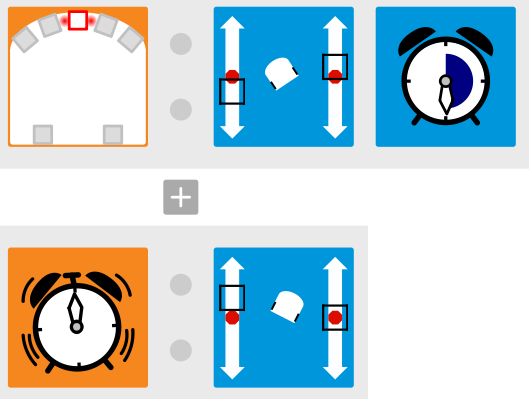
\includegraphics[width=.4\textwidth]{shy} &
\begin{minipage}[b]{.5\textwidth}
\begin{footnotesize}
\begin{verbatim}
  onevent prox
    when prox.horizontal[2] > 2000 do
      motor.left.target = -150
      motor.right.target = 100
      timer.period[0] = 2000
    end
  
  onevent timer0
    timer.period[0] = 0
    motor.left.target = 200
    motor.right.target = 0
\end{verbatim}
\end{footnotesize}
%\vspace*{1ex}
\end{minipage}
\end{tabular}
\end{center}

Le robot Thymio a deux minuteurs.
Vous pouvez changer la durée d'un minuteur en affectant une valeur aux entrées 0 ou 1 du
tableau \p{timer.period}.
La valeur est en \emph{millisecondes}, c'est-à-dire en millièmes de secondes.
Pour régler le minuteur 0 sur 2 secondes, la valeur 2000 (millisecondes) doit être 
affectée à \p{timer.period[0]}.

Il y a deux événements, \p{timer0} et \p{timer1} (<<\,timer\,>> signifie <<\,minuteur\,>> en anglais),
un pour chacun des minuteurs.
Lorsque la durée est écoulée, l'événement \textit{timer} est déclenché.
Dans le traitement d'événement \p{timer0}, on remet la durée du timer à 0 pour que l'événement
ne se redéclenche plus et on change la vitesse des moteurs.

Dans l'initialisation, le programme règle le minuteur sur 0 pour éviter qu'événement ne se déclenche
par accident au début du programme:

\begin{footnotesize}
\begin{verbatim}
  # stop timer 0
  timer.period[0] = 0
\end{verbatim}
\end{footnotesize}

\newpage

\sect{États}

Les \cref{ch.states,ch.counting} ont montré comment utiliser les \emph{états}.
Le robot Thymio peut être dans 16 états différents et on peut spécifier dans quel état précis 
le robot doit être pour qu'un certain événement déclenche une certaine action.
Dans le programme \p{count-to-two.aesl} du \cref{ch.counting}, l'état est mis à 0 lorsque
le bouton central est touché.
Il compte ensuite si le nombre de frappes des mains est pair ou impair en altérnant entre
l'état 0 et l'état 1.
Le programme VPL et le traitement d'événement AESL pour le bouton central sont:
\footnote{Le programme AESL montré ici est différent de celui généré par VPL pour des raisons
qui seront expliquées plus bas dans ce chapitre.}

\begin{center}
\begin{tabular}{ll}
\raisebox{8ex}{
\includegraphics[width=.4\textwidth]{two-button}} &
\begin{minipage}[b]{.5\textwidth}
\begin{footnotesize}
\begin{verbatim}
  var state[] = [0,0,0,0]
  
  onevent buttons
    when button.center == 1 do
      state[0] = 0
      state[1] = 0
      state[2] = 0
      state[3] = 0
    end
\end{verbatim}
\end{footnotesize}
\end{minipage}
\end{tabular}
\end{center}

L'état mémorisé dans le tableau \p{state[]} contient 4 éléments.
Chaque élément peut prendre les valeurs 0 ou 1.
Il y a donc $2\times2\times2\times2=16$ différentes valeurs possible pour ce tableau.
On initialise ces éléments du tableau à 0 en affectant les 4 valeurs {\footnotesize\verb+[0,0,0,0]+}.
La valeur initiale du tableau est aussi utilisée pour déduire le nombre d'éléments du tableau;
comme il y a quatre valeurs dans {\footnotesize\verb+[0,0,0,0]+},
il y aura quatre éléments dans le tableau.

Le bloc événement état (en vert, à côté du bloc événement bouton) a les quatres quartiers en gris;
cela signifie que l'événement aura lieu indépendamment de l'état actuel.
Ainsi, à chaque fois que le bouton central est touché, le bloc événement action (en bleu) change
l'état actuel à 0 pour tous les éléments du tableau \p{state}, comme indiqué par les quartiers blancs.
Dans le programme AESL correspondant, la structure \p{when} vérifie si le bouton central a été touché,
mais ne vérifie pas les valeurs contenues dans le tableau \p{state}.
Si le bouton central a été touché, chaque élément du tableau est remis à 0.

Il y a deux blocs événement frapper des mains, associés à des blocs état différents.
Dans le programme textuel, un seul traitement d'événement \p{mic} est utilisé.
Les instructions à exécuter seront déterminées à l'aide de structures \p{if} (\cref{fig.respond}).

\begin{figure}[hbt]
\begin{center}
\begin{tabular}{ll}
\raisebox{10ex}{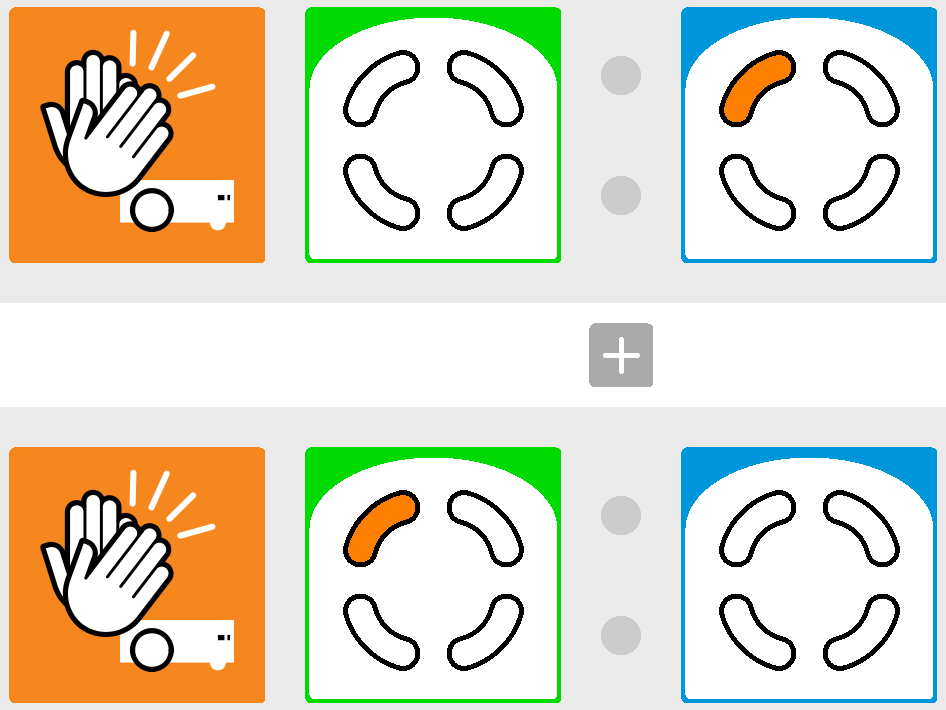
\includegraphics[width=.4\textwidth]{two-clap}} &
\begin{minipage}[b]{.5\textwidth}
\begin{footnotesize}
\begin{verbatim}
  onevent mic
    if state[0] == 0 and
       state[1] == 0 and
       state[2] == 0 and
       state[3] == 0 then
      state[0] = 1
      state[1] = 0
      state[2] = 0
      state[3] = 0
    end
    if state[0] == 1 and
       state[1] == 0 and
       state[2] == 0 and
       state[3] == 0 then
      state[0] = 0
      state[1] = 0
      state[2] = 0
      state[3] = 0
    end
\end{verbatim}
\end{footnotesize}
\end{minipage}
\end{tabular}
\caption{Réagir aux frappes des mains selon l'état actuel}\label{fig.respond}
\end{center}
\end{figure}

La signification du mot-clé \p{and} (<<\,et\,>> en anglais) est que \emph{toutes} les conditions dans 
la structure \p{if} doivent être vérifiées pour que les instructions entre le
\p{then} et le \p{end} soient exécutées.
Si tous les éléments du tableau \p{state} sont 0, on affecte la valeur 1 à l'élément \p{state[0]},
tandis que l'on affecte la valeur 0 aux autres éléments.
Ceci correspond à un bloc événement état avec tous les quartiers blancs
et à un bloc action état avec le quartier supérieur gauche orange et les autres blancs.
De même, si la valeur de \p{state[0]} est 1 et les valeurs des autres éléments est 0,
les valeurs de tous les éléments de \p{state} sont remis à 0.

\newpage

\sect{Sous-routines}

Il arrive souvent qu'une même suite d'instructions doive être exécutée à plusieurs reprises
à des endroits différents du programme.
On pourrait écrire ces instructions une fois puis les copier chaque fois qu'on en a besoin.
Une solution plus simple consiste à utiliser une \emph{sous-routine}, qui permet
d'attribuer un nom à une suite d'instructions.
Dans ce programme, l'expression {\footnotesize\verb+sub display_state+} déclare une
sous-routine qui attribue au nom {\footnotesize\verb+display_state+} une suite d'instructions,
ici, une seul instruction, \p{call leds.circle}:

\bigskip

\begin{footnotesize}
\begin{verbatim}
  # subroutine to display the current state
  sub display_state
    call leds.circle(
      0, state[1]*32, 0, state[3]*32, 0, state[2]*32, 0, state[0]*32)
\end{verbatim}
\end{footnotesize}

Lorsque la sous-routine est \emph{appelée}, la suite d'instructions attribuée au nom de la sous-routine
est exécutée:
\vspace{-1ex}
\begin{footnotesize}
\begin{verbatim}
  callsub display_state
\end{verbatim}
\end{footnotesize}
\vspace{-1ex}
La fonction d'interface \p{leds.circle} permet de contrôler les huit LEDs entourant les boutons.
Là il faut vraiment vous référer au diagramme de la petite carte de référence pour apprendre
quel paramètre correspond à quelle LED!

L'intensité de chaque LED peut être contrôlée en donnant une valeur entre 0 (LED éteinte)
et 32 (LED complètement allumée).
Les LEDs avant, arrière, gauche et droite sont mises à 0 (éteintes), tandis que les LEDs diagonales
sont allumées si l'élément correspondant du tableau d'état est 1
et éteintes s'il est 0.
Pour obtenir ce résultat, on utilise les \emph{expressions arithmétiques} \p{state[...]*32}
qui multiplient la valeur des éléments du tableau par 32.
Si une des valeurs est 0, le résultat sera 0, tandis que si elle vaut 1, le résultat sera 32.

\newpage

\sect{Fonctions natives}

Le programme ci-dessus a un problème.
Puisque les valeurs des éléments du tableau \p{state} sont affectées une à une,
il est possible qu'un événement différent se produise
alors que les valeurs d'une partie des éléments ont été modifiées, mais pas de tous.
Pour modifier tous les éléments en même temps, il faut d'abord mettre les nouvelles valeurs
dans un nouveau tableau \p{new\_state} et puis les copier dans le premier tableau \p{state}:

\begin{footnotesize}
\begin{verbatim}
# variables for state
var state[4] = [0,0,0,0]
var new_state[4] = [0,0,0,0]

onevent buttons
  when button.center == 1 do
    new_state[0] = 0
    new_state[1] = 0
    new_state[2] = 0
    new_state[3] = 0
  end
  
  call math.copy(state, new_state)
  callsub display_state
\end{verbatim}
\end{footnotesize}

La \emph{fonction native} \p{math.copy} est utilisée pour copier des tableaux.
Les fonctions natives sont déjà intégrées dans le robot Thymio et sont plus efficaces
que des suites d'instructions dans AESL.
Les fonctions natives sont décrites dans la documentation d'Aseba.

La version actuelle d'AESL autorise les affectations de tableaux entiers, de telle sorte qu'il
aurait été possible d'utiliser une instruction d'affectation:
\footnote{L'affectation de tableaux se traduit en fait par une suite d'affectations individuelles,
élément par élément, de sorte qu'il n'y a aucun d'intérêt à utiliser une affectation de tableau.}

\begin{footnotesize}
\begin{verbatim}
  state = new_state
\end{verbatim}
\end{footnotesize}
